
\documentclass[12pt]{article}

\newcommand{\VERSION}{1.7.4}

\usepackage[utf8]{inputenc}
\usepackage[english]{babel}
\usepackage{csquotes}

\usepackage{xcolor}
\usepackage{listings, lstautogobble}

\usepackage{graphicx}
\graphicspath{{../figures/}}

\lstset{language=bash,
	keywordstyle=\color{black},
	basicstyle=\small\ttfamily,
	commentstyle=\ttfamily\itshape\color{gray},
	stringstyle=\ttfamily,
	showstringspaces=false,
	breaklines=true,
	frameround=ffff,
	frame=single,
	rulecolor=\color{black},
	autogobble=true
}

\usepackage{hyperref}
\hypersetup{
	colorlinks=true,
	linktoc=all,
	linkcolor=blue,
	citecolor=blue
}

\begin{document}
	
	\title{DTarray\_pro installation and basic usage}
	\author{Aaron Maurais}
	\date{24 September 2018}
	
	\maketitle
	\tableofcontents
	%\newpage
	
	\section{Introduction}
	
	\texttt{DTarray\_pro} extracts Uniprot ID numbers, molecular weights, and spectral counts from DTASelect-filter files. Protein data is combined into one dataset and written to the working directory as a tab delimitated text file (.tsv). This document will describe how to install and use the latest version of \texttt{DTarray\_pro} step by step. Some experience using a unix shell is assumed.  
		
	\section{Installation}
	
	\texttt{DTarray\_pro} is hosted at GitHub, which is a free hosting service for distributed version control in software development.  
	The latest stable version of \texttt{DTarray\_pro} will be posted at \url{https://github.com/ajmaurais/DTarray_pro/releases}
	
	\subsection{Download and unpack DTarray\_pro archive file from GitHub}
	\begin{itemize}
		\item Navigate to the \href{https://github.com/ajmaurais/DTarray_pro/releases}{releases} tab on the \texttt{DTarray\_pro} GitHub page.
		
		\item The files for the latest release should be at the top of the page.
		
		\item Download the file: \texttt{Source code (tar.gz)} for the latest release, to you computer.
		
		\item \texttt{DTarray\_pro} expects to be installed in \texttt{\textasciitilde/local}. The program needs data stored in text files in \texttt{\textasciitilde/local/DTarray\_pro-\VERSION/db} for some features to work. First make the directory \texttt{\textasciitilde/local} on your \texttt{pleiades} account if it doesn't already exist.
		
		\item Transfer the source code archive (should be named something like \texttt{DTarray\_pro-\VERSION.tar}) to your \texttt{pleiades} account using your FTP client of choice.	
		
		\item The source code archive has to be unpacked before you can access it. To unpack the \texttt{.tar} type the following commands in your terminal.
		
		\begin{lstlisting}
			$ cd ~/local
			$ tar -xfv DTarray_pro-1.7.4.tar
		\end{lstlisting}
		
		\item As a result, a new directory should be created in \texttt{~/local} named \texttt{DTarray\_pro-\VERSION}
		
		\item Once you have unpacked the archive, you no longer need the \texttt{.tar} file and can delete if of you wish.
		
	\end{itemize}

	\subsection{Build DTarray\_pro executable}
	\begin{itemize}
		\item Before you can use \texttt{DTarray\_pro}, you have to build the executable from source. Fortunately \texttt{DTarray\_pro} is configured to work with a build automation tool called \texttt{make} so the process should be straightforward.
		
		\item To build \texttt{DTarray\_pro} run the following commands in your terminal.
		
		\begin{lstlisting}
			$ cd ~/local/DTarray_pro-1.7.4/
			$ ./configure
			$ make
		\end{lstlisting}
		
		\item After you have run \texttt{make}, there should be several new files in the \texttt{DTarray\_pro-\VERSION} directory.  If everything worked, the executable file should be located at \texttt{DTarray\_pro-\VERSION/bin/DTarray}
		
	\end{itemize}

	\subsection{Adding a shortcut for DTarray\_pro (optional)}
	
	To run \texttt{DTarray\_pro} you have to navigate on your terminal to a folder which contains DTASelect-filter files then type the full path to the executable file relative from the directory you are currently in.  Its possible to install a program system wide so you don't have to type the path every time, but without administrative privileges, its a bit complicated. A workaround is to create a shortcut or alias to the executable file.  This section will explain how to add an alias for \texttt{DTarray\_pro} to your shell profile on \texttt{pleiades}
	
	\begin{itemize}
		\item To add an alias for \texttt{DTarray\_pro}, you will have to edit your shell profile, which is a file stored in your home directory named \texttt{.tcshrc}.
		
		\item To edit your shell profile, you will use a command line text editor called \texttt{nano}. To open \texttt{.tcshrc} in \texttt{nano}, type:
		
		\begin{lstlisting}
			$ cd
			$ nano .tcshrc
		\end{lstlisting}
		
		\item After starting \texttt{nano}, your terminal window should look something like this:
		
		\begin{figure}[h!]
			\centering
			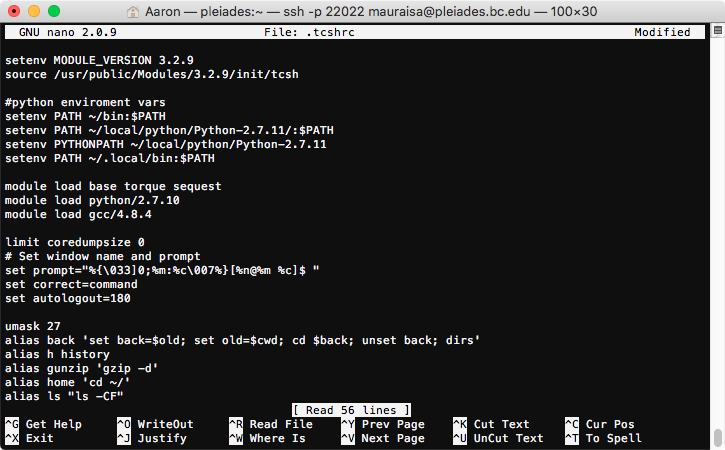
\includegraphics[width=0.7\textwidth]{step_1.png}
		\end{figure}
		
		\item Scroll to the bottom of the file and add the line: \\ \texttt{alias DTarray "\textasciitilde/local/DTarray\_pro-1.7.4/bin/DTarray"}
		
		\begin{figure}[h!]
			\centering
			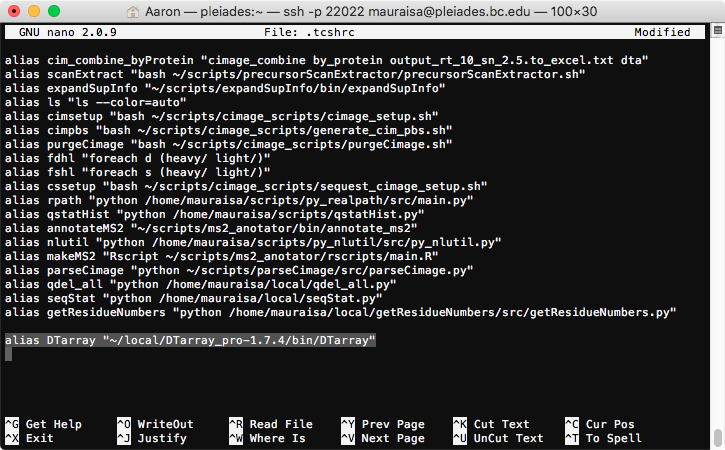
\includegraphics[width=0.8\textwidth]{step_2.png}
		\end{figure}
	
		\item To save and exit the file, hit \texttt{\textasciicircum + X}. A dialog should show up at the bottom which says: 
		\begin{lstlisting}
			Save modified buffer (ANSWERING "No" WILL DESTROY CHANGES) ?
		\end{lstlisting}
		\item Hit \texttt{y}
		
		\item Next a dialog should show up at the bottom which says 
		
		\begin{lstlisting}
			File name to write: .tcshrc
		\end{lstlisting}
		
		\item Hit \texttt{enter} to exit.
		
		\item Finally you have to tell the computer to reload your shell profile after you have modified it with the command:
		
		\begin{lstlisting}
			$ source .tcshrc
		\end{lstlisting}
		
		\item You can test your alias by typing the following command from your home directory:
		
		\begin{lstlisting}
			$ DTarray --version
		\end{lstlisting}
		
		\item If the alias is recognized by the computer, it should display something like:
		
		\begin{lstlisting}
			DTarray_pro 1.7
			Last git commit: Sat Sep 22 20:28:17 2018
			git revision: 04d30f4fd7790abfca60197d85cefc9d2a877cfc
		\end{lstlisting}
		
	\end{itemize}
	
	\section{Usage}
	
	\subsection{Input format options}
	
	Users have two options for how the input DTASelect-filter files passed to \texttt{DTarray\_pro} are structured.  
	
	\subsubsection{std mode} 
		
	In \texttt{std} mode, DTASelect-filter are stored in a common directory and the files are named with the format \texttt{<sample\_name>.dtafilter} (This is the default input mode for \texttt{DTarray\_pro}.)
	
	\begin{lstlisting}
		$ ls
		sample_1.dtafilter		sample_2.dtafilter
		sample_3.dtafilter		sample_4.dtafilter
	\end{lstlisting}
	
	The user can either manually setup the 
		
		%\item \textbf{subdir} mode, where 
	
	\subsubsection{subidr mode}
	
	In \texttt{subdir} mode, DTASelect-filter files are stored in a separate directory, the directory name is the sample name, and the filter files are named \texttt{DTASelect-filter.txt} (This is the default input mode for \texttt{dtarray.pl}.)
	
	\begin{lstlisting}
		$ find */*.txt
		sample_1/DTASelect-filter.txt
		sample_2/DTASelect-filter.txt
		sample_3/DTASelect-filter.txt
		sample_4/DTASelect-filter.txt
	\end{lstlisting}
	
\end{document}
